\section{Simulations and discussion}\label{sec:sim}

\subsection{Set-up}
We use the example of~\citet{juchem2027restoring}: $(\tau,\sigma)=(11,9)$,
$n=0.2010$, $(\Op,\Om)=(1.1055,0.9045)$\,rad/s, $P_0=62.52$\,s, $v_0=1$
($\Hr=0.5$).
The realised loop has the following imperfections:
\begin{itemize}
\item controller period $T_s=0.03$\,s;
\item one-sample sensor and actuator delays (0.03\,s each);
\item sensor gain error $-3\,\%$ and actuator gain error $+6.5\,\%$;
\item additive sensor noise $\mathcal N(0,0.002^2)$ on $q$ and $\dot q$;
\item actuator backlash (play) of half-width $0.003$.
\end{itemize}
By \cref{prop:zoh}, $\deq=0.09$\,s.
The simulator propagates host and virtual oscillator \emph{exactly} between
samples under \cref{ass:sampled}, so no integration error enters the
comparison.
The modal coordinates are reconstructed with the projector of the frozen system
$A(n+c_\psi,\omega_z)$.
For the ECC loop, which retunes $\omega_z$, the frequency estimate uses the
least-squares slope of the unwrapped modal phases over batches of one $P_0$ in
place of I/Q demodulation.
All code is in the accompanying repository (\texttt{code/}).

Five configurations are compared:
\begin{itemize}
\item uncompensated;
\item energy loop only ($K_E=10$);
\item energy and amplitude loops ($K_E=10$, $K_A=1$),
  as in~\citet{juchem2027restoring};
\item the full ECC hierarchy with $\omega_z$ adaptation ($K_\Omega=1$);
\item the proposed controller \eqref{eq:control}, with $K_E=10$, $K_A=1$,
  $k_{IA}=0.02$, $k_P=0.02$, $k_I=2\times10^{-4}$, and the phase loop switched
  on at $t=200$\,s.
\end{itemize}
Metrics are evaluated over the last $25\,\%$ of a $3000$\,s run.
The table lists the RMS errors, the frequency-ratio error $|\hat r-\tau/\sigma|$,
the median over common periods of the per-period minimum of $H_q/\Hr$, and the
closure error $\varepsilon_{\mathrm{cl}}$ of~\citet{juchem2027restoring}.
The closure error uses the period inferred from the estimated modal lines.

\begin{table*}[t]
  \centering
  \caption{Late-time performance (last 25\,\% of 3000\,s). The ratio error is not
  reported when one mode dominates ($\mathrm{RMS}|\eA|>1$).
  The per-period minimum measures recurrent depletion, not a one-off near miss.}
  \label{tab:metrics}
  % generated by code/scripts/run_simulations.py -- do not edit by hand
\begin{tabular}{lccccc}
\toprule
Case & RMS $|e_H|$ & RMS $|e_A|$ & $|\hat r-\tau/\sigma|$ & $\mathrm{med}_j\min H_q/H_r$ & $\varepsilon_{\mathrm{cl}}$\\
\midrule
Nominal (ideal) & $0$ & $0$ & $0$ & $0$ & $0$\\
Uncompensated & $9.2{\times}10^{13}$ & $3.66$ & -- & $1.3{\times}10^{12}$ & $0.14$\\
Energy ($u$) & $0.0383$ & $3.19$ & -- & $0.496$ & $8.7{\times}10^{-5}$\\
Energy--amplitude ($u,s$) & $0.0436$ & $0.0316$ & $3.5{\times}10^{-3}$ & $4.9{\times}10^{-4}$ & $7.6{\times}10^{-3}$\\
ECC: $u,s,\omega_z$ [batch] & $0.0462$ & $0.345$ & $3.8{\times}10^{-4}$ & $1.7{\times}10^{-5}$ & $0.0885$\\
Proposed: $u,s$+PI, trim $c$ & $0.0436$ & $0.0238$ & $7.5{\times}10^{-6}$ & $1.2{\times}10^{-5}$ & $2.5{\times}10^{-4}$\\
\bottomrule
\end{tabular}

\end{table*}

\subsection{Results}
\Cref{tab:metrics} and \cref{fig:sim-portraits,fig:sim-errors} summarise the
results.
Without compensation the fast mode grows at the rate predicted by
\cref{thm:delay,prop:zoh} and the energy diverges.
The energy loop alone bounds the energy but leaves $\eA\approx3.2$: one mode
carries almost all of the energy, the phase portrait is close to a circle, and
the subsystem energies are nearly stationary.
Adding the amplitude loop restores deep exchange but leaves a residual
$\eA\approx0.03$.
This is the steady state $S\alpha_\Sigma/K_A=0.018$ of \cref{lem:averaged} plus
measurement bias, and the uncontrolled relative phase drifts.

The ECC frequency loop drives the measured ratio close to $\tau/\sigma$ on
average, but $\omega_z$ never converges.
It hunts between $1.02$ and $1.07$ (\cref{fig:sim-errors}(e)), on and beyond the
point $\sqrt{1+\kappa}\approx1.02$ where its authority vanishes.
This is the behaviour predicted by \cref{prop:authority}, since here
$\kappa>n^2+n^4/4$.
The relative phase keeps wandering, so the per-period host minimum fluctuates by
two orders of magnitude and the closure error rises to $0.09$.

The proposed controller locks $\psi$ to $\psis$ within a few hundred seconds.
The trim converges to $c_\psi\approx-\eta_c$, as predicted by
\cref{thm:iss-avg}(c).
The integral action removes the mean of $\eA$, which drops to $O(10^{-4})$.
The ratio error drops to $7.5\times10^{-6}$ and the closure error to
$2.5\times10^{-4}$.
\emph{Every} common period now reaches $H_q/\Hr\approx1.2\times10^{-5}$.
This is about forty times deeper than the energy--amplitude configuration, and
it is achieved recurrently rather than at isolated instants.
The residual $\eH\approx0.04$ is the bias that the $-3\,\%$ sensor gain
induces in $\hat H$ (\cref{thm:iss-avg}(a)); it is a measurement limit, not a
control limit.

\begin{figure*}[t]
  \centering
  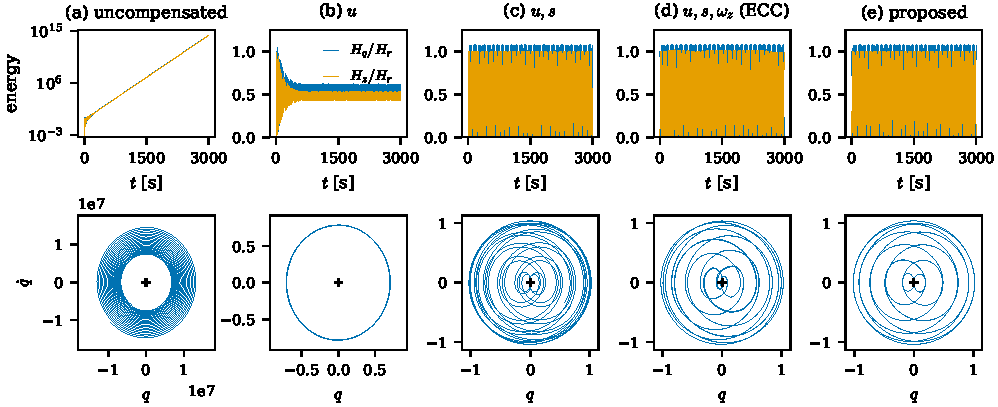
\includegraphics[width=\textwidth]{fig_sim_portraits.pdf}
  \caption{Subsystem energies (top) and host phase plane over the last two common
  periods (bottom) for the successive configurations under delay, ZOH, gain
  errors, noise and backlash. (a) Divergence; (b) bounded energy but one
  dominant mode; (c) deep exchange, drifting phase; (d) hunting $\omega_z$ loop;
  (e) phase-locked closed orbit.}
  \label{fig:sim-portraits}
\end{figure*}

\begin{figure*}[t]
  \centering
  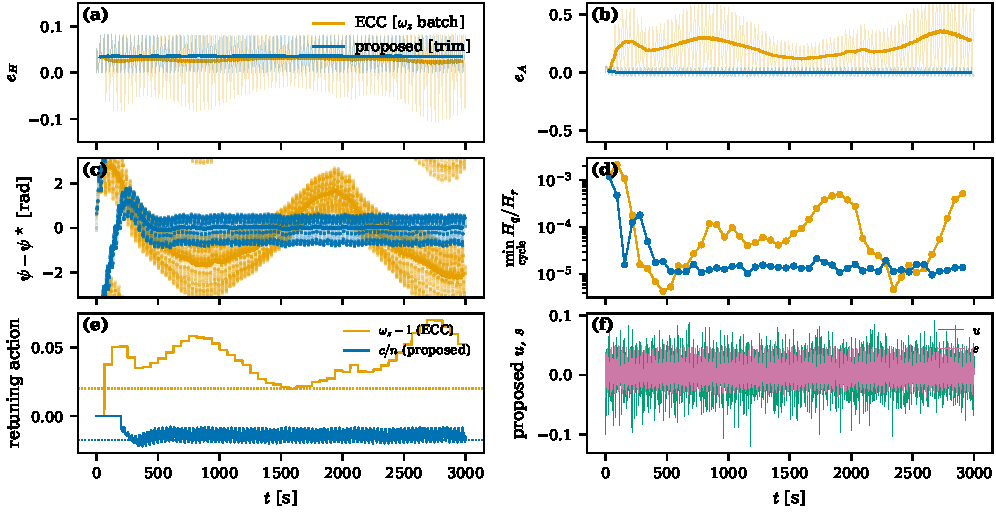
\includegraphics[width=\textwidth]{fig_sim_errors.pdf}
  \caption{ECC hierarchy (orange) versus proposed controller (blue). Faint: raw
  signals; solid: means over $P_0$. (a) $\eH$; (b) $\eA$; (c) relative phase
  error; (d) per-period minimum of $H_q/\Hr$; (e) retuning actions $\omega_z-1$
  and $c_\psi/n$, with the authority limit $\sqrt{1+n^2}-1$ and the predicted
  trim $-\eta_c/n$ dotted; (f) fast actions $u$, $s$ of the proposed
  controller.}
  \label{fig:sim-errors}
\end{figure*}

\subsection{Discussion and limitations}
\paragraph*{Which imperfections matter}
\Cref{thm:delay,prop:zoh,prop:static} rank the mechanisms.
Delay and hold create first-order modal anti-damping, which no static gain error
does, and their effect scales with $\deq=(1+k_y+k_a)T_s$.
The single most effective hardware measure is therefore to reduce the loop
latency.

\paragraph*{Phase ripple}
The relative phase shows a fast ripple of about $0.5$\,rad around its locked
mean (\cref{fig:sim-errors}(c)).
The phase $\psi$ amplifies modal-phase errors by $\tau$ and $\sigma$, and part
of the ripple is due to noise and to the residual mode mixing caused by delay and
backlash.
At the apex target this ripple costs only quadratically (\cref{rem:apex}).
\gap{Phase estimation}{Quantify the ripple sources (noise, mode mixing from
delay/backlash, fast $u$, $s$), compare the instantaneous projector with I/Q
demodulation~\citep{franks1969signal}, and filter $\hat\psi$ if useful. The
CRB argument of~\citet{juchem2027restoring} applies to frequency, not to the
phase measured here.}

\paragraph*{Dissipation and reference energy}
The controller redistributes energy; at the absorption instants the host is at
rest and the energy resides in software.
A practical device will remove it there, e.g.\ by resetting or damping the
virtual oscillator, and then re-arm.
\gap{Harvesting and reference energy}{Specify the harvesting stage and its
interaction with the loops. If the host has small physical damping,
regulating $H$ to the fixed $\Hr$ injects energy; replace $\Hr$ by a decaying or
estimated reference and check that \cref{thm:iss-avg} survives.}

\paragraph*{Fairness of the ECC comparison}
\gap{Baseline}{The ECC loop is reproduced with a phase-slope frequency estimator
instead of I/Q demodulation; confirm with the original estimator that the
hunting is structural (\cref{prop:authority}) rather than an estimator
artefact. Also add a passivity-based baseline (time-domain passivity
control~\citep{hannaford2002time}) for completeness.}

\paragraph*{Experiment}
\gap{Experimental validation}{A single-DOF set-up (voice-coil actuated
mass--spring or a cantilever with a co-located shaker) would strengthen the
paper considerably. Without it, the theory has to carry the contribution.}
